% Chapter Template

\chapter{Matrix Mode Corrections} % Main chapter title

\label{Chapter 5} % Change X to a consecutive number; for referencing this chapter elsewhere, use \ref{ChapterX}

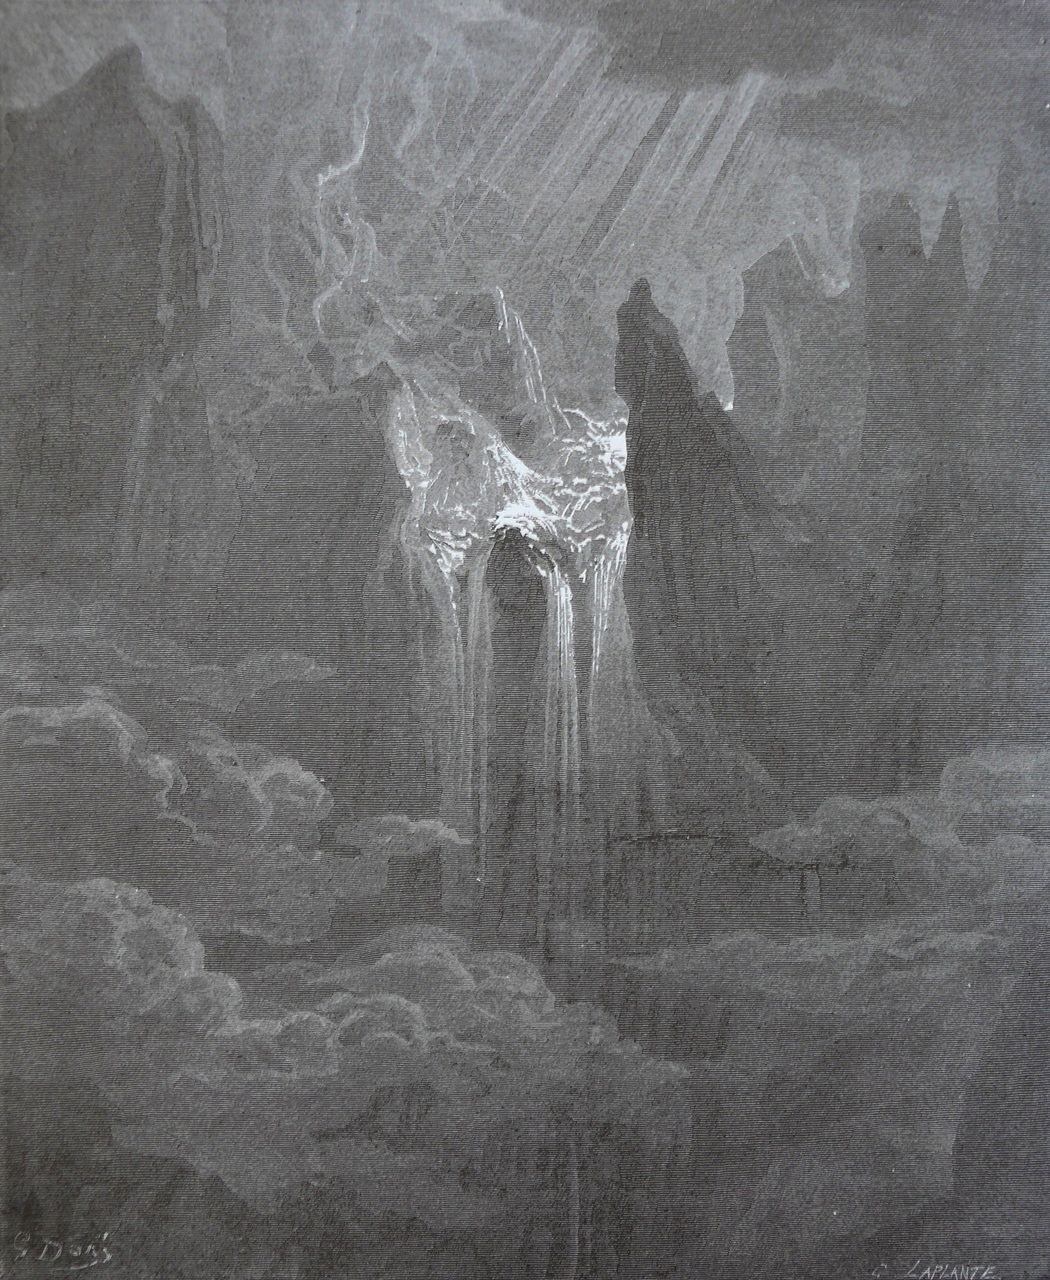
\includegraphics[width=\linewidth,trim={0 16cm 0 3cm},clip]{Paradise_Lost_30}

\section{Overview}

In the following chapter the issues discovered in matrix mode are outlined, analysed and then the solutions to the problems are described. This begins with the serial interface locking issue and then moves onto the uart monitor, matrix mode compositor handshaking issue. The letterboxing implementation is then discussed and the chapter is ended with the smaller bug fixes to matrix mode.

%----------------------------------------------------------------------------------------
%	SECTION 1
%----------------------------------------------------------------------------------------

\section{Serial Locking}

\label{Ch5 Sec1}

One existing issue with the phone was that when it entered matrix mode, the serial interface with the board would lock up. This would render all attempts at interfacing with the MEGA65 useless. Locking the serial input to the device was expected whilst in matrix mode, as this would prevent subversion of during sensitive program execution. The failure to return serial functionality to the device upon leaving matrix mode was showed that there was some handshaking protocols that were not behaving as expected.This phenomenon was especially strange as the code to disable the serial input while in matrix mode was removed for debug purposes. This proved that it was not entering or exiting matrix mode that caused the bug, but some protocol within the character processing or character displaying.

%-----------------------------------
%	SUBSECTION 1
%-----------------------------------
\subsection{Creating the Test-bench}

\label{Ch5 Sec1 Sub1}

Due to the long synthesis times, in excess of an hour, a light weight version of the phone needed to be created. Thanks to debugging in the past, this problem had already been encountered and solved. In order to save time during synthesis previously, a version of the phone was created without the CPU. This version was outdated and required some additional ports to spoof the components into working correctly. A CPU free version of the phone, some of which can be seen in figures \ref{fig:nocpuzero}, \ref{fig:nocpuone}, \ref{fig:nocputwo}, was possible thanks to matrix mode being composited over the video feed in hardware, rather than being done in software. Once the CPU free components were working, a Vivado technical command language (tcl) file was acquired from one of the other contributors to the project. This file was used to set up and execute the vivado tasks required to create and compile the CPU-less version of the phone. This resulted in a bit stream that was able to be run on the Nexys4ddr boards in the lab.

\begin{figure}
  \centering
  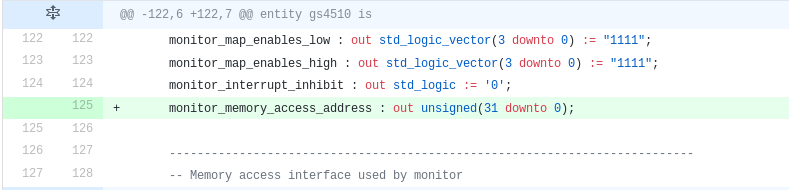
\includegraphics[width=\linewidth]{nocpuzero}
  \caption{Addition of monitor memory access address port to the nocpu.vhdl file.}
  \label{fig:nocpuzero}
\end{figure}

\begin{figure}
  \centering
  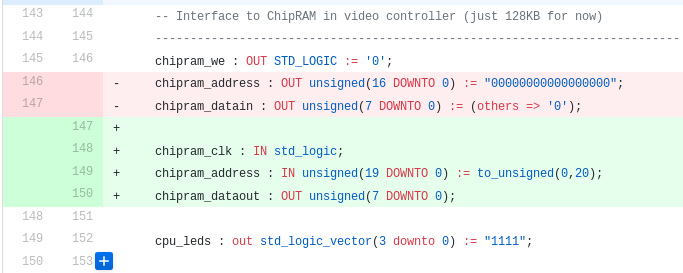
\includegraphics[width=\linewidth]{nocpuone}
  \caption{Addition of the chip ram clock and modification to the chip ram address and data ports in nocpu.vhdl.}
  \label{fig:nocpuone}
\end{figure}

\begin{figure}
  \centering
  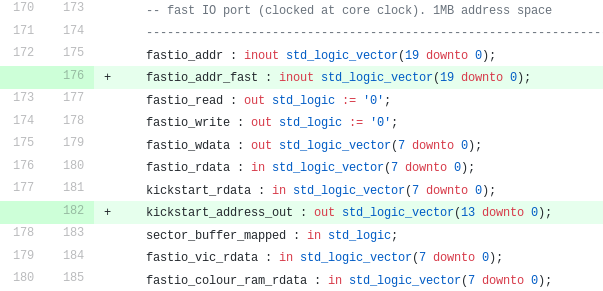
\includegraphics[width=\linewidth]{nocputwo}
  \caption{Fast I/O address port and kickstart address port additions to the nocpu.vhdl file.}
  \label{fig:nocputwo}
\end{figure}

%-----------------------------------
%	SUBSECTION 2
%-----------------------------------
\subsection{Timing Issues}

\label{Ch5 Sec1 Sub2}

One of the theorised causes for the serial locking issue was that the timing between the handshaking protocols was misaligned and was causing a state in which the serial output was not able to be read. In order to find these issues a timing report needed to be generated during synthesis. This was achieved by altering the tcl file and enabling the timing report generation, as seen in figure \ref{fig:timing}. This change was done to all of the tcl files as it would allow any type of synthesis, no CPU or otherwise, to generate timing reports. This would assist in identifying when signals that extend synthesis due to timing issues in the future. In the timing reports generated, several video signals were found to be causing timing issues; to solve these an intermediary signal was created to host the video data. As seen in figure \ref{fig:videodelay}, this would cause the data to be delayed by one clock cycle, the loss in time was determined to be acceptable as the difference of a pixel appearing a clock cycle late would not be perceptible to the human eye. This fix was not just applied to the vga signal, it was also applied to some signals in the frame generator, pixel mapper, io mapper and top level assembly. Some of the signals that were causing timing issues were unable to be driven, this was because they were determined to be critical. These signals required if statement reduction to reduce the logic delay between the source and destination registers. This was as the delay between the source and destination caused values in the outer statements to become stale before the inner logic could be resolved. In order to perform these reductions, the arguments in the inner statements were merged into the outer statements. Unfortunately, the resolution of the timing issues had no impact on the serial locking, but it did result in faster synthesis and a clearer image on the screen.

\begin{figure}
  \centering
  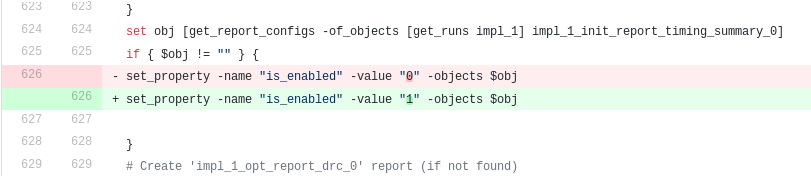
\includegraphics[width=\linewidth]{timing}
  \caption{The tcl file change that allowed the generation of timing reports.}
  \label{fig:timing}
\end{figure}

\begin{figure}
  \centering
  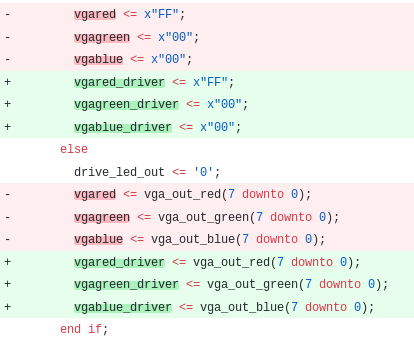
\includegraphics[width=\linewidth]{videodelay}
  \caption{Addition of vga driving signals to the viciv.vhdl file.}
  \label{fig:videodelay}
\end{figure}

%-----------------------------------
%	SUBSECTION 3
%-----------------------------------
\subsection{Handshaking Issues}

\label{Ch5 Sec1 Sub3}

As the timing issues were cleared, it was determined that the locking issue must be an error in the handshaking rather than a signal error. Firstly the keycode data that was passed from the terminal emulator to the rain compositor, as well as the iomapper key data and terminal emulator state were examined. This was done via the seven segment display on the nexys4ddr development board, as seen in figure \ref{fig:segleddata}. This revealed that the correct data was being passed prior to matrix mode and even after the lock had occurred. Further more, it showed that the terminal emulator was getting stuck in the print banner stage, in which, a predefined string was sent to the rain compositor. This suggested that the rest of the terminal emulator was working correctly and it was the output function that was causing the issue. Removing the printing section from the print banner state resulted in the serial output not locking up upon leaving matrix mode.\\

After further examining some of the flags associated with the output character function, it was noted that the terminal emulator would set two flags when sending characters, as seen in figure \ref{fig:outputchar}. The first is the character valid flag, it was observed to go high after a single character input and then never go low between subsequent inputs. This was also true for the second flag, the terminal emulator just sent flag. Looking for other instances of the both flags revealed that they were supposed to be reset while the terminal emulator was not ready, as seen in figure \ref{fig:termemureadyzero}. This terminal emulator ready flag was followed into the matrix rain compositor and it was discovered that the terminal emulator was only not ready when scrolling or when processing a character in the specific case seen in figure \ref{fig:termemureadytwo}. As these cases were correctly setting the terminal emulator to not ready when it was busy, the handshaking error was determined to be in the statement seen in figure \ref{fig:termemureadyzero}. Examining figure \ref{fig:termemureadyzero}, figure \ref{fig:termemureadytwo} and figure \ref{fig:outputchar} together, it can be seen that there is a logic clash when sending a character. The output character function sets the just sent and character valid flags high, which is then used to set the ready flag low, which is used to set the just sent and character valid flags low. This error was corrected by flipping the reset logic, as seen in figure \ref{fig:termemureadyone}. This resulted in matrix mode no longer locking up the serial input after processing a single character.

\begin{figure}
  \centering
  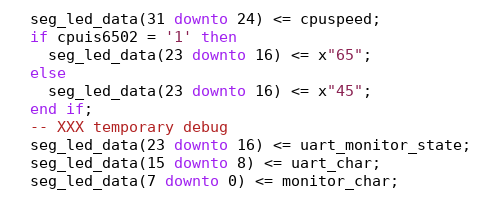
\includegraphics[width=\linewidth]{segleddata}
  \caption{Temporary debug output added to enable keyboard and serial keycode and terminal emulator state visualisation.}
  \label{fig:segleddata}
\end{figure}

\begin{figure}
  \centering
  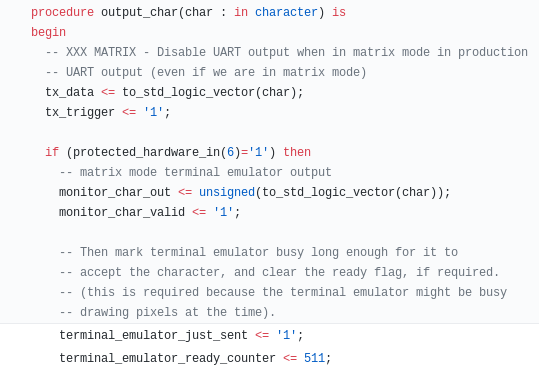
\includegraphics[width=\linewidth]{outputchar}
  \caption{The output character function within the uart monitor subsystem.}
  \label{fig:outputchar}
\end{figure}

\begin{figure}
  \centering
  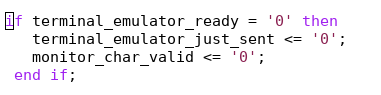
\includegraphics[width=\linewidth]{termemureadyzero}
  \caption{The monitor character valid and terminal emulator just sent flag reset statement.}
  \label{fig:termemureadyzero}
\end{figure}

\begin{figure}
  \centering
  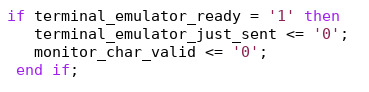
\includegraphics[width=\linewidth]{termemureadyone}
  \caption{The corrected monitor character valid and terminal emulator just sent flag reset statement.}
  \label{fig:termemureadyone}
\end{figure}

\begin{figure}
  \centering
  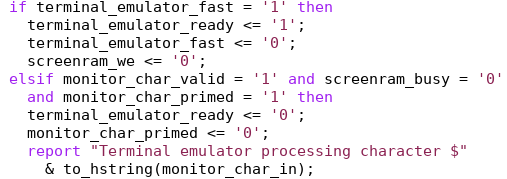
\includegraphics[width=\linewidth]{termemureadytwo}
  \caption{The matrix rain compositor character sequencing code.}
  \label{fig:termemureadytwo}
\end{figure}

%----------------------------------------------------------------------------------------
%	SECTION 2
%----------------------------------------------------------------------------------------

\section{Letterboxing}

\label{Ch5 Sec2}

One of the issues with matrix mode was that the matrix mode overlay was exceeding the desired bounds. This resulted in junk data to be loaded into the areas of the screen that were supposed to be blank. It also caused the top of the matrix mode display to appear above the visible portion of the screen and the end of matrix mode the continue off the screen, all of which can be seen in figure \ref{fig:noletterbox}.

%-----------------------------------
%	SUBSECTION 1
%-----------------------------------

\subsection{Makefile Correction}

\label{Ch5 Sec2 Sub1}

When looking at the error it was believed the the junk data was caused by rouge input from somewhere, as this input was always the same, it was determined to be some predefined string. Through an examination of matrix mode, it was discovered that the only source of input to the mode was the terminal emulator. Disconnecting the terminal emulator from the matrix rain compositor did not have any effect on the junk data being displayed however. This confirmed that the issue was not with the input to matrix mode, but in the compositor itself. Following the input characters into the matrix mode compositor lead to the case statement that handles the character processing and in particular, the case seen in figure \ref{fig:mmcharacterhandeling}. The monitor character can be seen being assigned to the screen ram write data, this write data signal is then used to write to the terminal memory, as seen in figure \ref{fig:mmscreenram}. This terminal memory, as seen by the use of screenram\_rdata in figure \ref{fig:mmtermmemout}, is then used to load character bits, which are then used to output characters to the screen. A joint examination of the terminal memory file with Dr. Gardner-Stephen, revealed that there were many preinitilized values in it via hardware. This was done in the makefile and the loaded values were the ASCII font and the matrix banner text. Removing both these from the terminal memory resolved the issue, but also resulted in no characters being able to be displayed. Further examination of the character set by Dr. Gardner-Stephen showed that two copies of it were being loaded into the terminal emulator and that one character set only required memory from location \$000 to location \$500. In order to remove this second character set from the terminal memory, after the character set was loaded, zeros were loaded into the address locations from \$800 to \$4095. This change, as seen in figure \ref{fig:termmemzeroing}, resulted in the matrix compositor only displaying unwanted characters in the lower portion of the screen. Figure \ref{fig:noletterboxromcorrection} shows change in issue, the remaining junk characters are either from the character set itself or the banner, both of which are unable to be removed from the terminal memory.

\begin{figure}
  \centering
  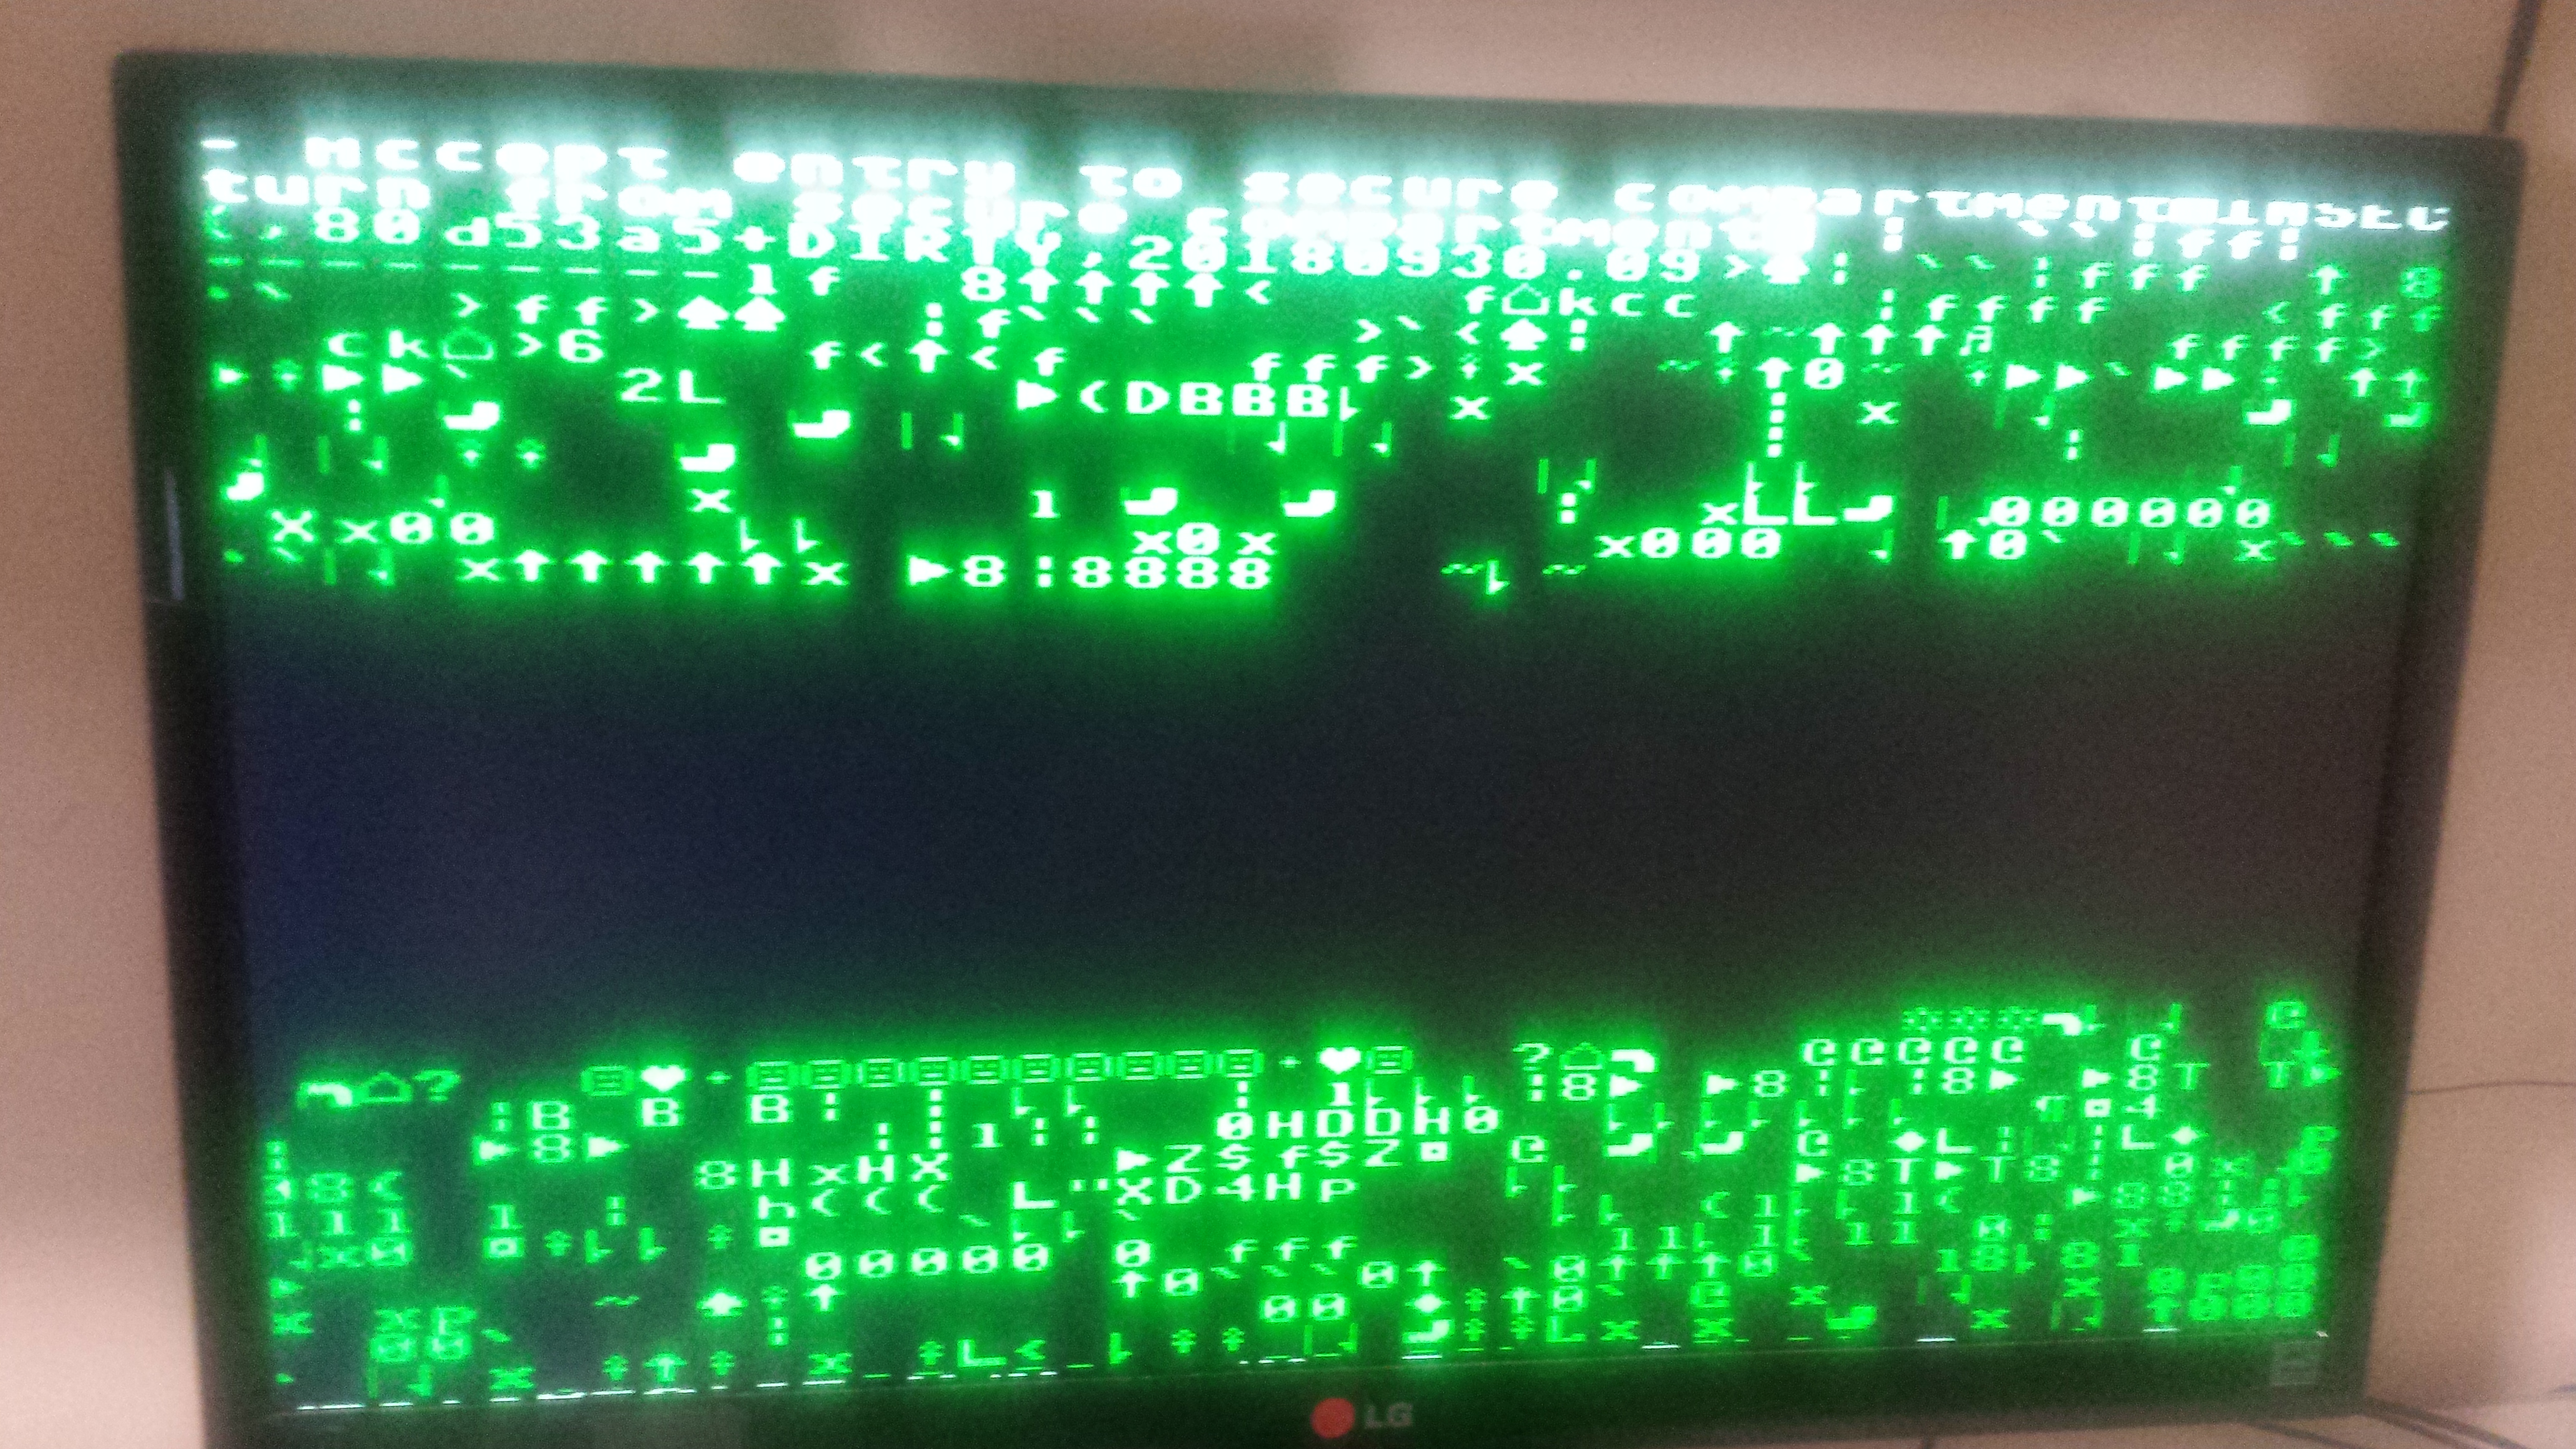
\includegraphics[width=\linewidth]{noletterbox}
  \caption{Matrix mode prior to letterbox fixes.}
  \label{fig:noletterbox}
\end{figure}

\begin{figure}
  \centering
  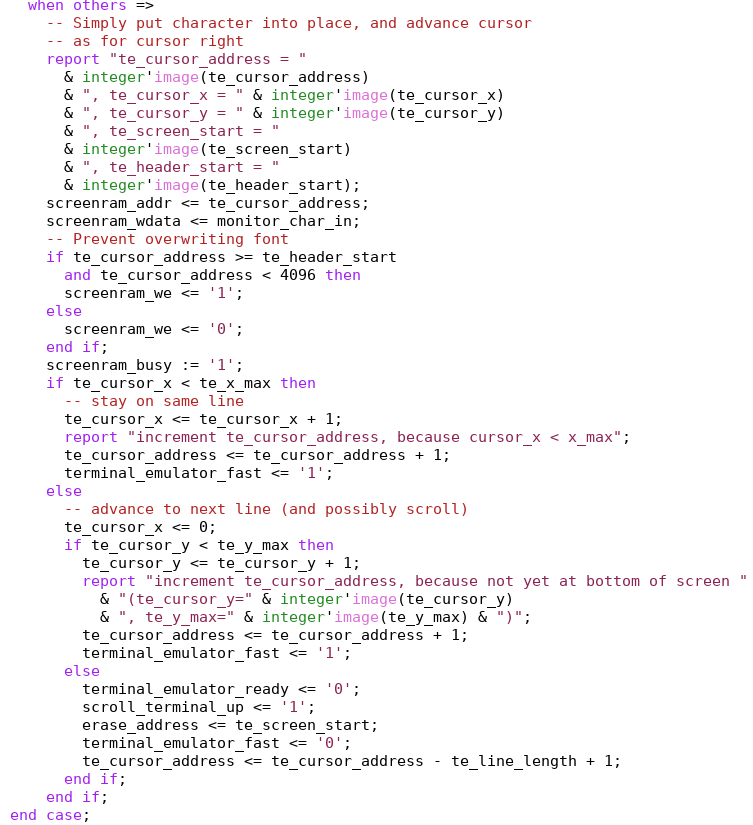
\includegraphics[width=\linewidth]{mmcharacterhandeling}
  \caption{The matrix rain compositor character processing code.}
  \label{fig:mmcharacterhandeling}
\end{figure}

\begin{figure}
  \centering
  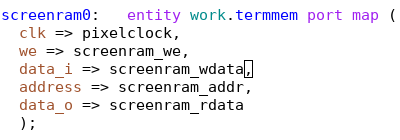
\includegraphics[width=\linewidth]{mmscreenram}
  \caption{The matrix mode screen ram entity.}
  \label{fig:mmscreenram}
\end{figure}

\begin{figure}
  \centering
  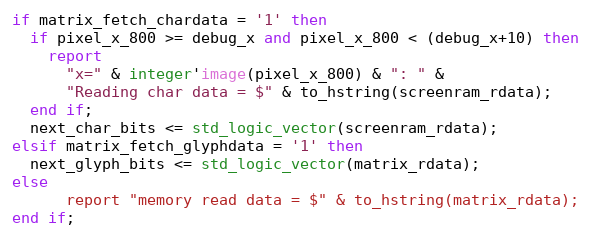
\includegraphics[width=\linewidth]{mmtermmemout}
  \caption{The assignment of the character bits in the terminal memory to the output variable.}
  \label{fig:mmtermmemout}
\end{figure}

\begin{figure}
  \centering
  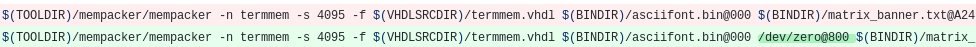
\includegraphics[width=\linewidth]{termmemzeroing}
  \caption{The makefile change to remove the excess character set from the terminal memory.}
  \label{fig:termmemzeroing}
\end{figure}

\begin{figure}
  \centering
  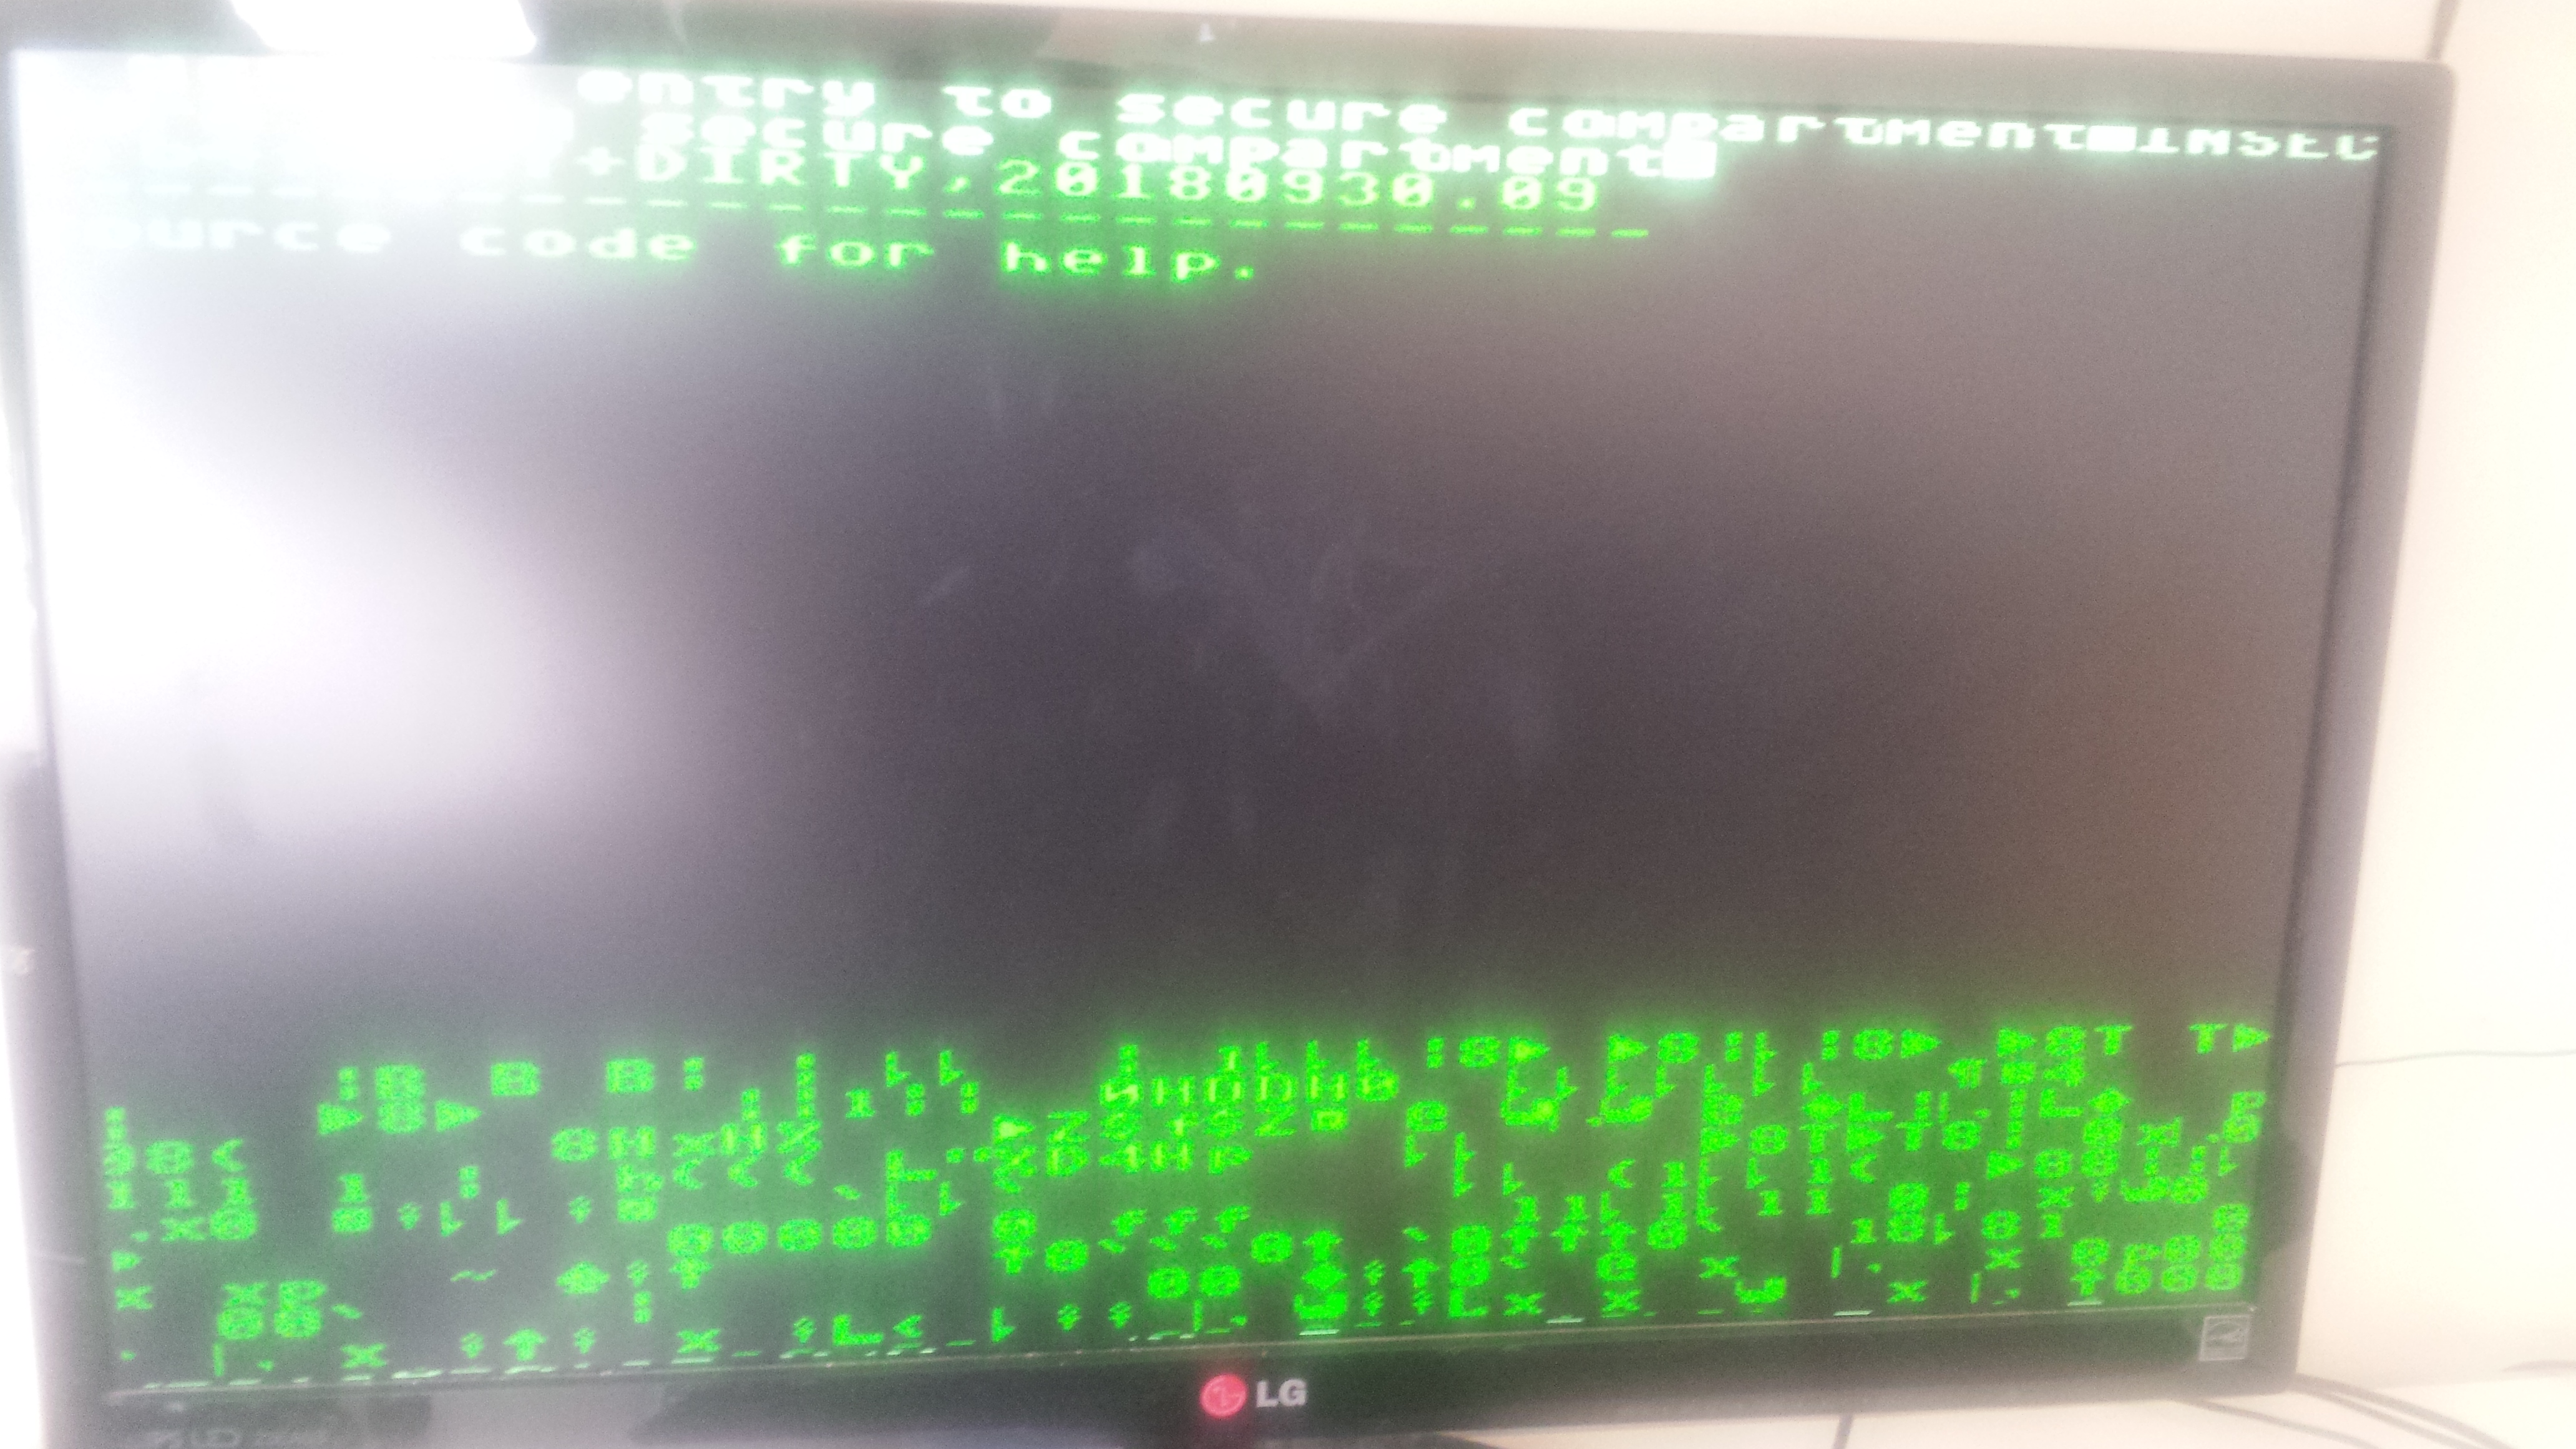
\includegraphics[width=\linewidth]{noletterboxromcorrection}
  \caption{Matrix mode without the second character set loaded into memory during compilation.}
  \label{fig:noletterboxromcorrection}
\end{figure}

%-----------------------------------
%	SUBSECTION 2
%-----------------------------------

\subsection{Letterbox Implementation}

\label{Ch5 Sec2 Sub2}

As the matrix mode display was still exceeding the desired bounds, a limiting signal was used to keep the visible output within a letterbox. One such signal already existed in the viciv and was being used for a similar purpose with the vga output. This signal was taken from the viciv and sent to the matrix mode compositor, where it was used in place of vsync. As seen in figure \ref{fig:letterboxcode}, in addition to the replacement of vsync, the letterbox signal was used to blank the region outside of the letterbox, this can be seen in figure \ref{fig:letterbox}. While the letterbox fixed the issues, it introduced some more minor issues into matrix mode. These issues are further discussed in the following sections.

\begin{figure}
  \centering
  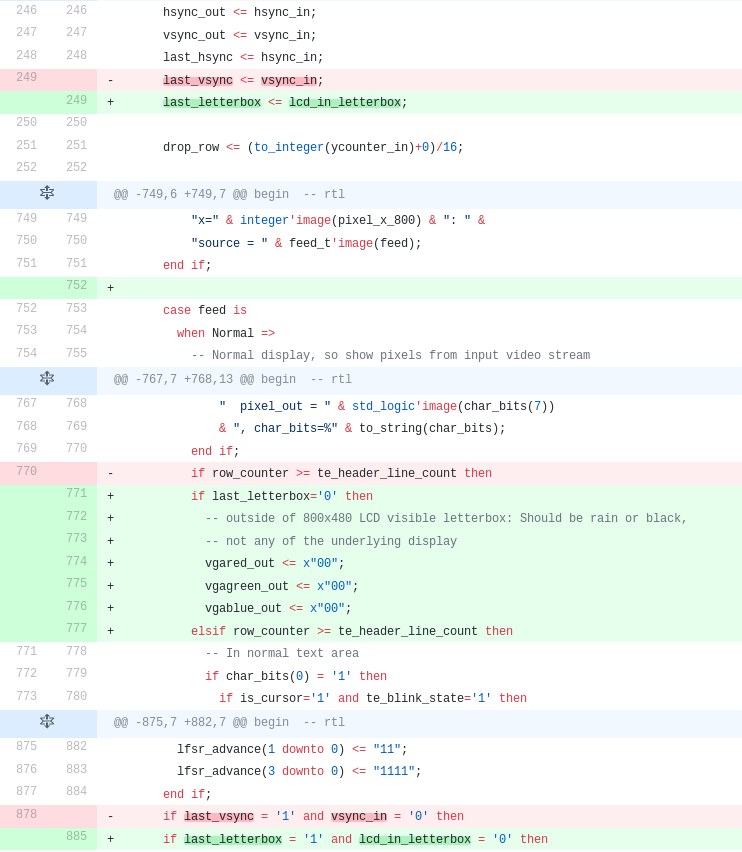
\includegraphics[width=\linewidth]{letterboxcode}
  \caption{The changes made to the matrix mode compositor to implement the letterboxing signal.}
  \label{fig:letterboxcode}
\end{figure}

\begin{figure}
  \centering
  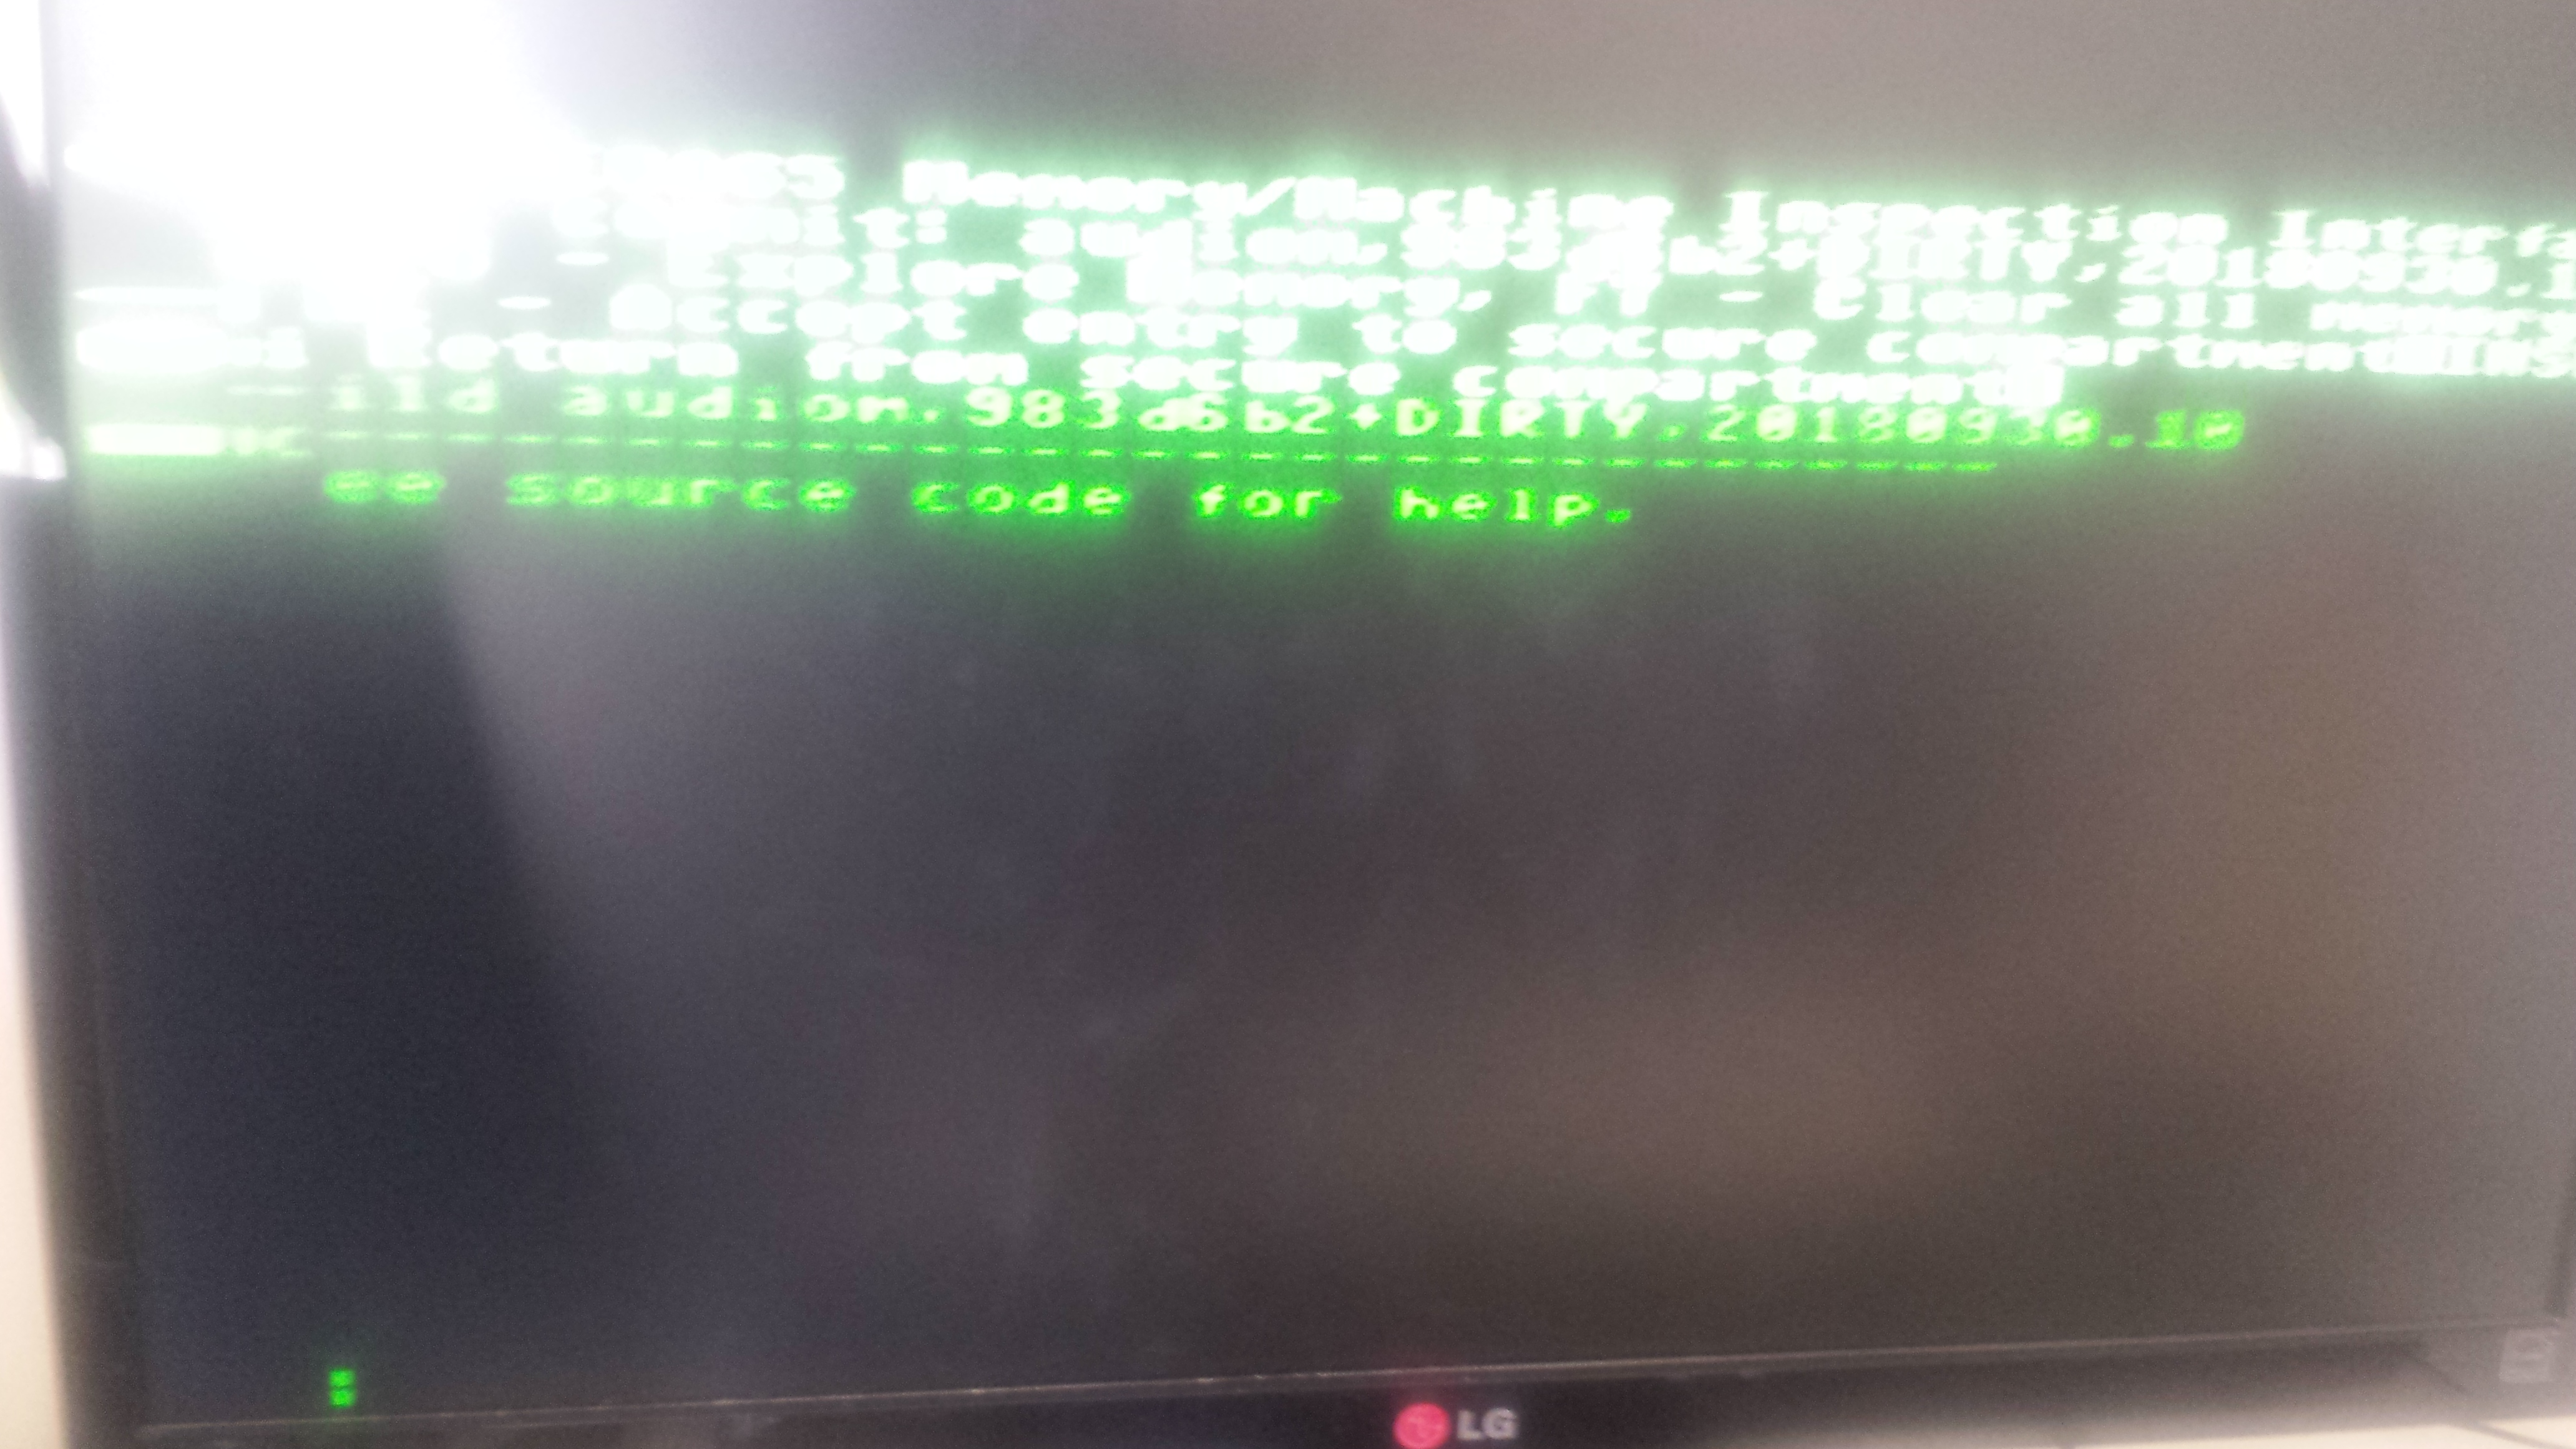
\includegraphics[width=\linewidth]{letterbox}
  \caption{Matrix mode with the letterboxing signal.}
  \label{fig:letterbox}
\end{figure}

%----------------------------------------------------------------------------------------
%	SECTION 4
%----------------------------------------------------------------------------------------

\section{Bug Fixing}

\label{Ch5 Sec3}

In addition to the matrix mode breaking bugs solved in sections \ref{Ch5 Sec1} and \ref{Ch5 Sec2}, there were also less urgent bugs in matrix mode that were solved. These bugs were graphical in nature and fixing them did not affect the overall functionality of matrix mode.

%-----------------------------------
%	SUBSECTION 1
%-----------------------------------

\subsection{Revolving Line}

\label{Ch5 Sec3 Sub1}

While restoring functionality to matrix mode it was noted that the input was not behaving as expected. A seen in figure \ref{fig:matrixmodelineinputerror}, whenever the cursor would go to a new line while scrolling it would move left one horizontal space. This resulted in the line revolving around the screen, this is believed to be due to under-flowing the horizontal position variable. Further examination of the variable, as seen in figure \ref{fig:revolvinglinezero} and figure \ref{fig:revolvinglineone}, show that during the new line handling while scrolling the cursor position is just rolled back to the start of the line. This does not take into account the full-stop used as an indication character at the start of each new line. The correction, as seen in figure \ref{fig:scrollline}, addresses this issue by starting the scrolled cursor position one increment to the right of the start of the line.

\begin{figure}
  \centering
  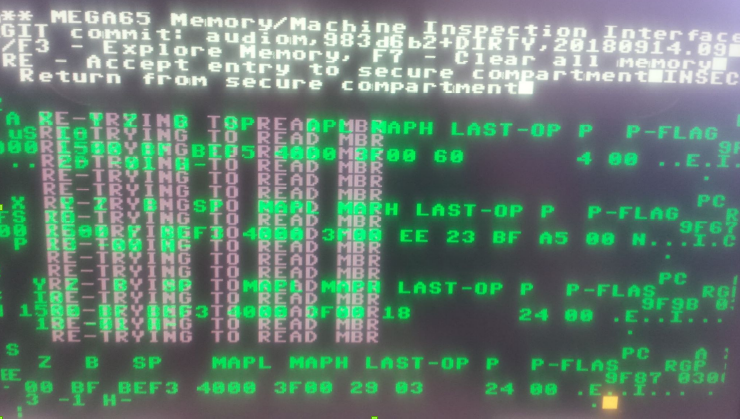
\includegraphics[width=\linewidth]{matrixmodelineinputerror}
  \caption{The matrix mode line revolution error.}
  \label{fig:matrixmodelineinputerror}
\end{figure}

\begin{figure}
  \centering
  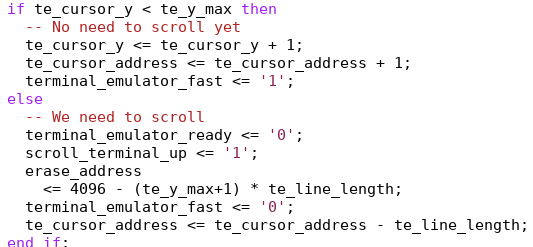
\includegraphics[width=\linewidth]{revolvinglinezero}
  \caption{The code used to handle the cursor address when scrolling in matrix mode.}
  \label{fig:revolvinglinezero}
\end{figure}

\begin{figure}
  \centering
  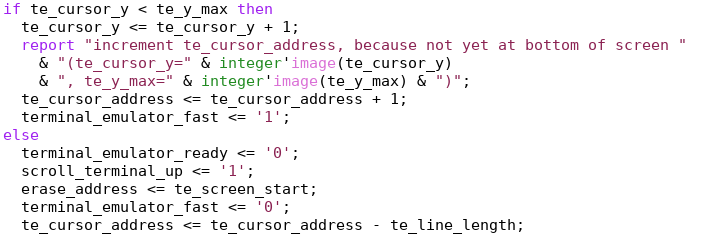
\includegraphics[width=\linewidth]{revolvinglineone}
  \caption{The code used when characters overflow onto the next line and scrolling is required.}
  \label{fig:revolvinglineone}
\end{figure}

\begin{figure}
  \centering
  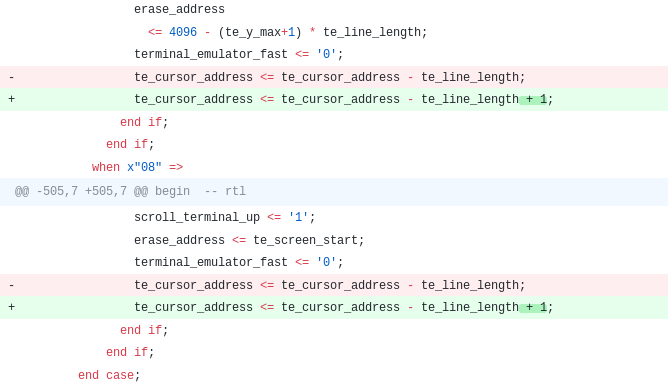
\includegraphics[width=\linewidth]{scrollline}
  \caption{The matrix rain compositor changes to eliminate the revolving line.}
  \label{fig:scrollline}
\end{figure}

%-----------------------------------
%	SUBSECTION 2
%-----------------------------------

\subsection{Bell Issue}

\label{Ch5 Sec3 Sub2}

During experimentation with the input to matrix mode it was noted that a strange character was being printed whenever the buffer overflowed. As identified by Dr. Gardner-Stephen, this character was intended to be the non printable bell character that would alert the user to an illegal action. This character can be seen as the "plus" symbols in figure \ref{fig:bellcharacter}. Examining the character output to the matrix mode compositor during when these bell characters were being output revealed that the key code being output was x"07". At the suggestion of Dr. Gardner-Stephen, an examination of the available keycodes showed that there was no case for this particular keycode. In order to stop this character from being printed, a case was added to handle it, as seen in figure \ref{fig:ignorebell}. This case would do nothing when it detected the bell character, this allowed for the character to be used later, while also preventing it from being printed. This introduced another error however, whenever a bell character was recognised it would lock up the input to matrix mode. This was due to the terminal emulator never being ready. Examination of the other cases showed that they all set terminal\_emulator\_fast to high after they had performed their case specific action. Implementing this, as seen in figure \ref{fig:newbell}, in the new case statement resulted in the issue being resolved.

\begin{figure}
  \centering
  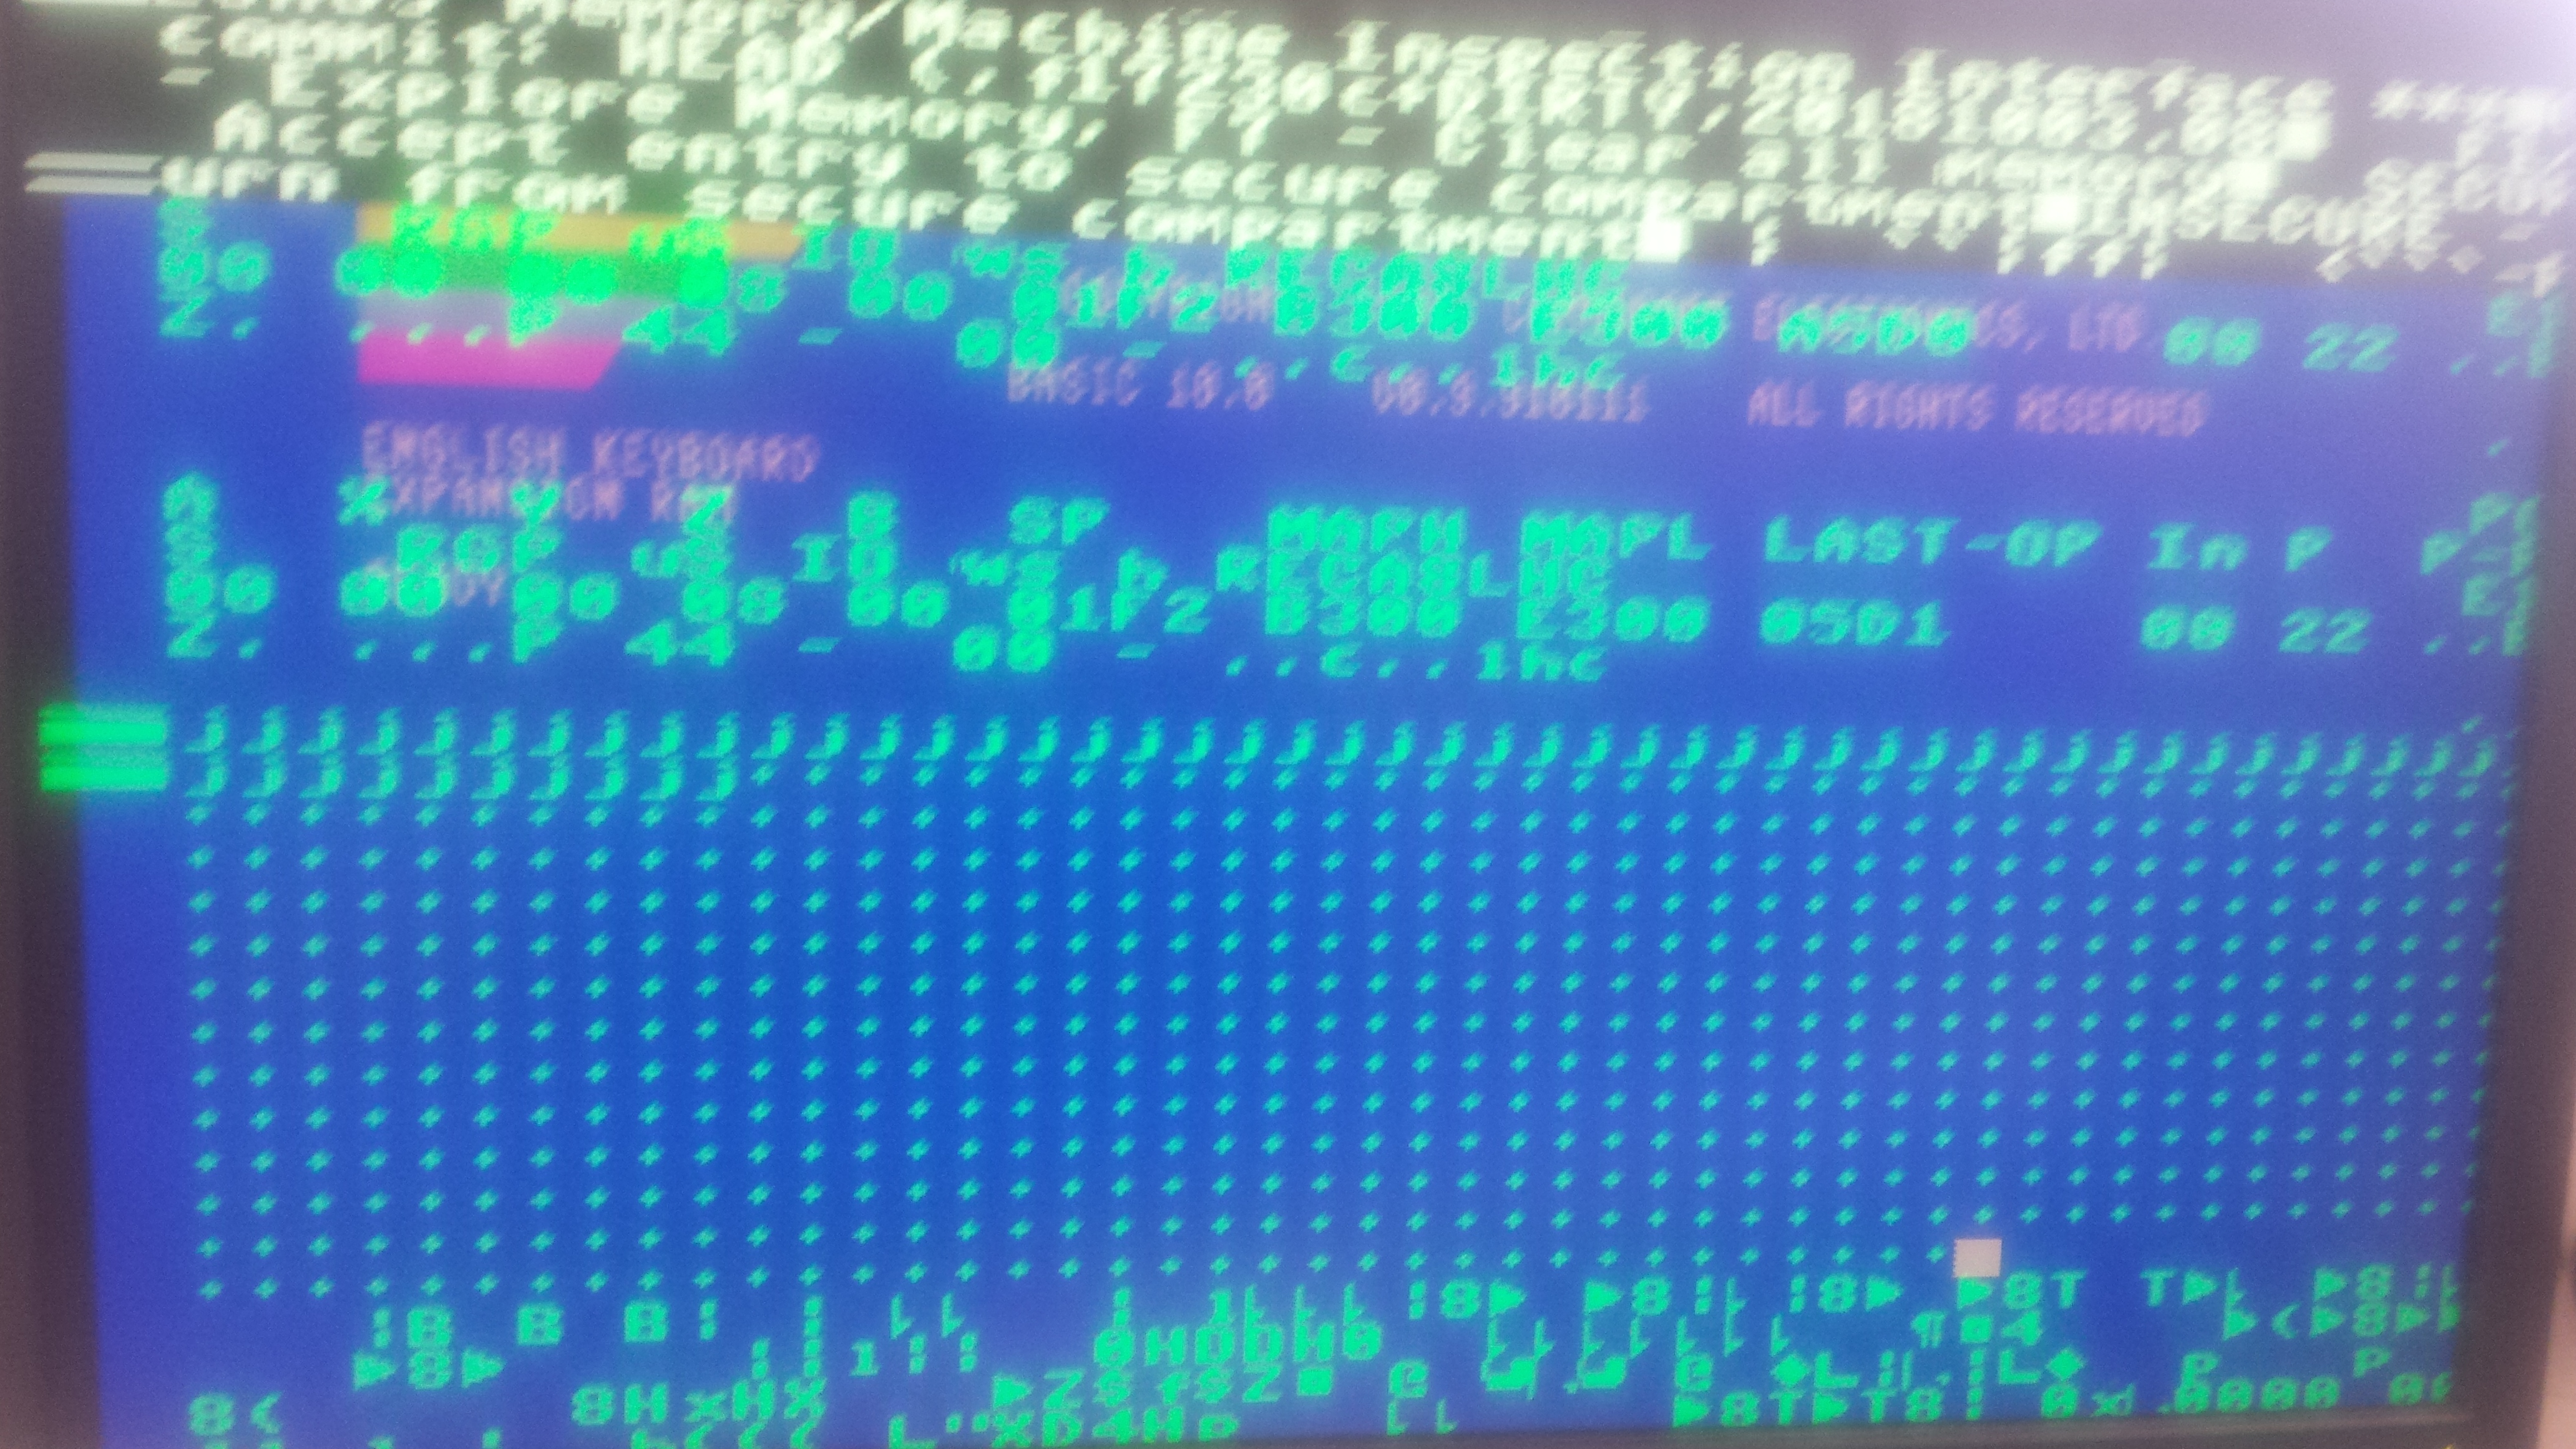
\includegraphics[width=\linewidth]{bellcharacter}
  \caption{The matrix mode with printed bell characters.}
  \label{fig:bellcharacter}
\end{figure}

\begin{figure}
  \centering
  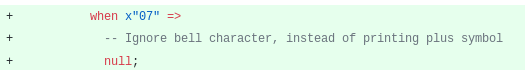
\includegraphics[width=\linewidth]{ignorebell}
  \caption{The case statement to ignore bell characters.}
  \label{fig:ignorebell}
\end{figure}

\begin{figure}
  \centering
  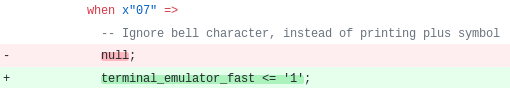
\includegraphics[width=\linewidth]{newbell}
  \caption{The change to the case statement to prevent serial locking.}
  \label{fig:newbell}
\end{figure}

%-----------------------------------
%	SUBSECTION 3
%-----------------------------------

\subsection{Pixel Shift}

\label{Ch5 Sec3 Sub3}

When examining the characters displayed to the screen, as noted in figure \ref{fig:biterror}, it was noted that some of them had their right most pixels wrapped around to the very left of the of the character tile. This output, as seen in figure \ref{fig:charbitstwo}, is due to the char\_bits variable. Tracing this variable back to its source revealed, as seen in figure \ref{fig:charbits}, that the bits for each character were being rotated around and used to decide whether to display a pixel or not. Dr. Garner-Stephen suggested, as the issue was a horizontal rotation, a rotation of the character bits should be performed, as displayed in figure \ref{fig:bitfix}. This fixed the pixel shift issue.

\begin{figure}
  \centering
  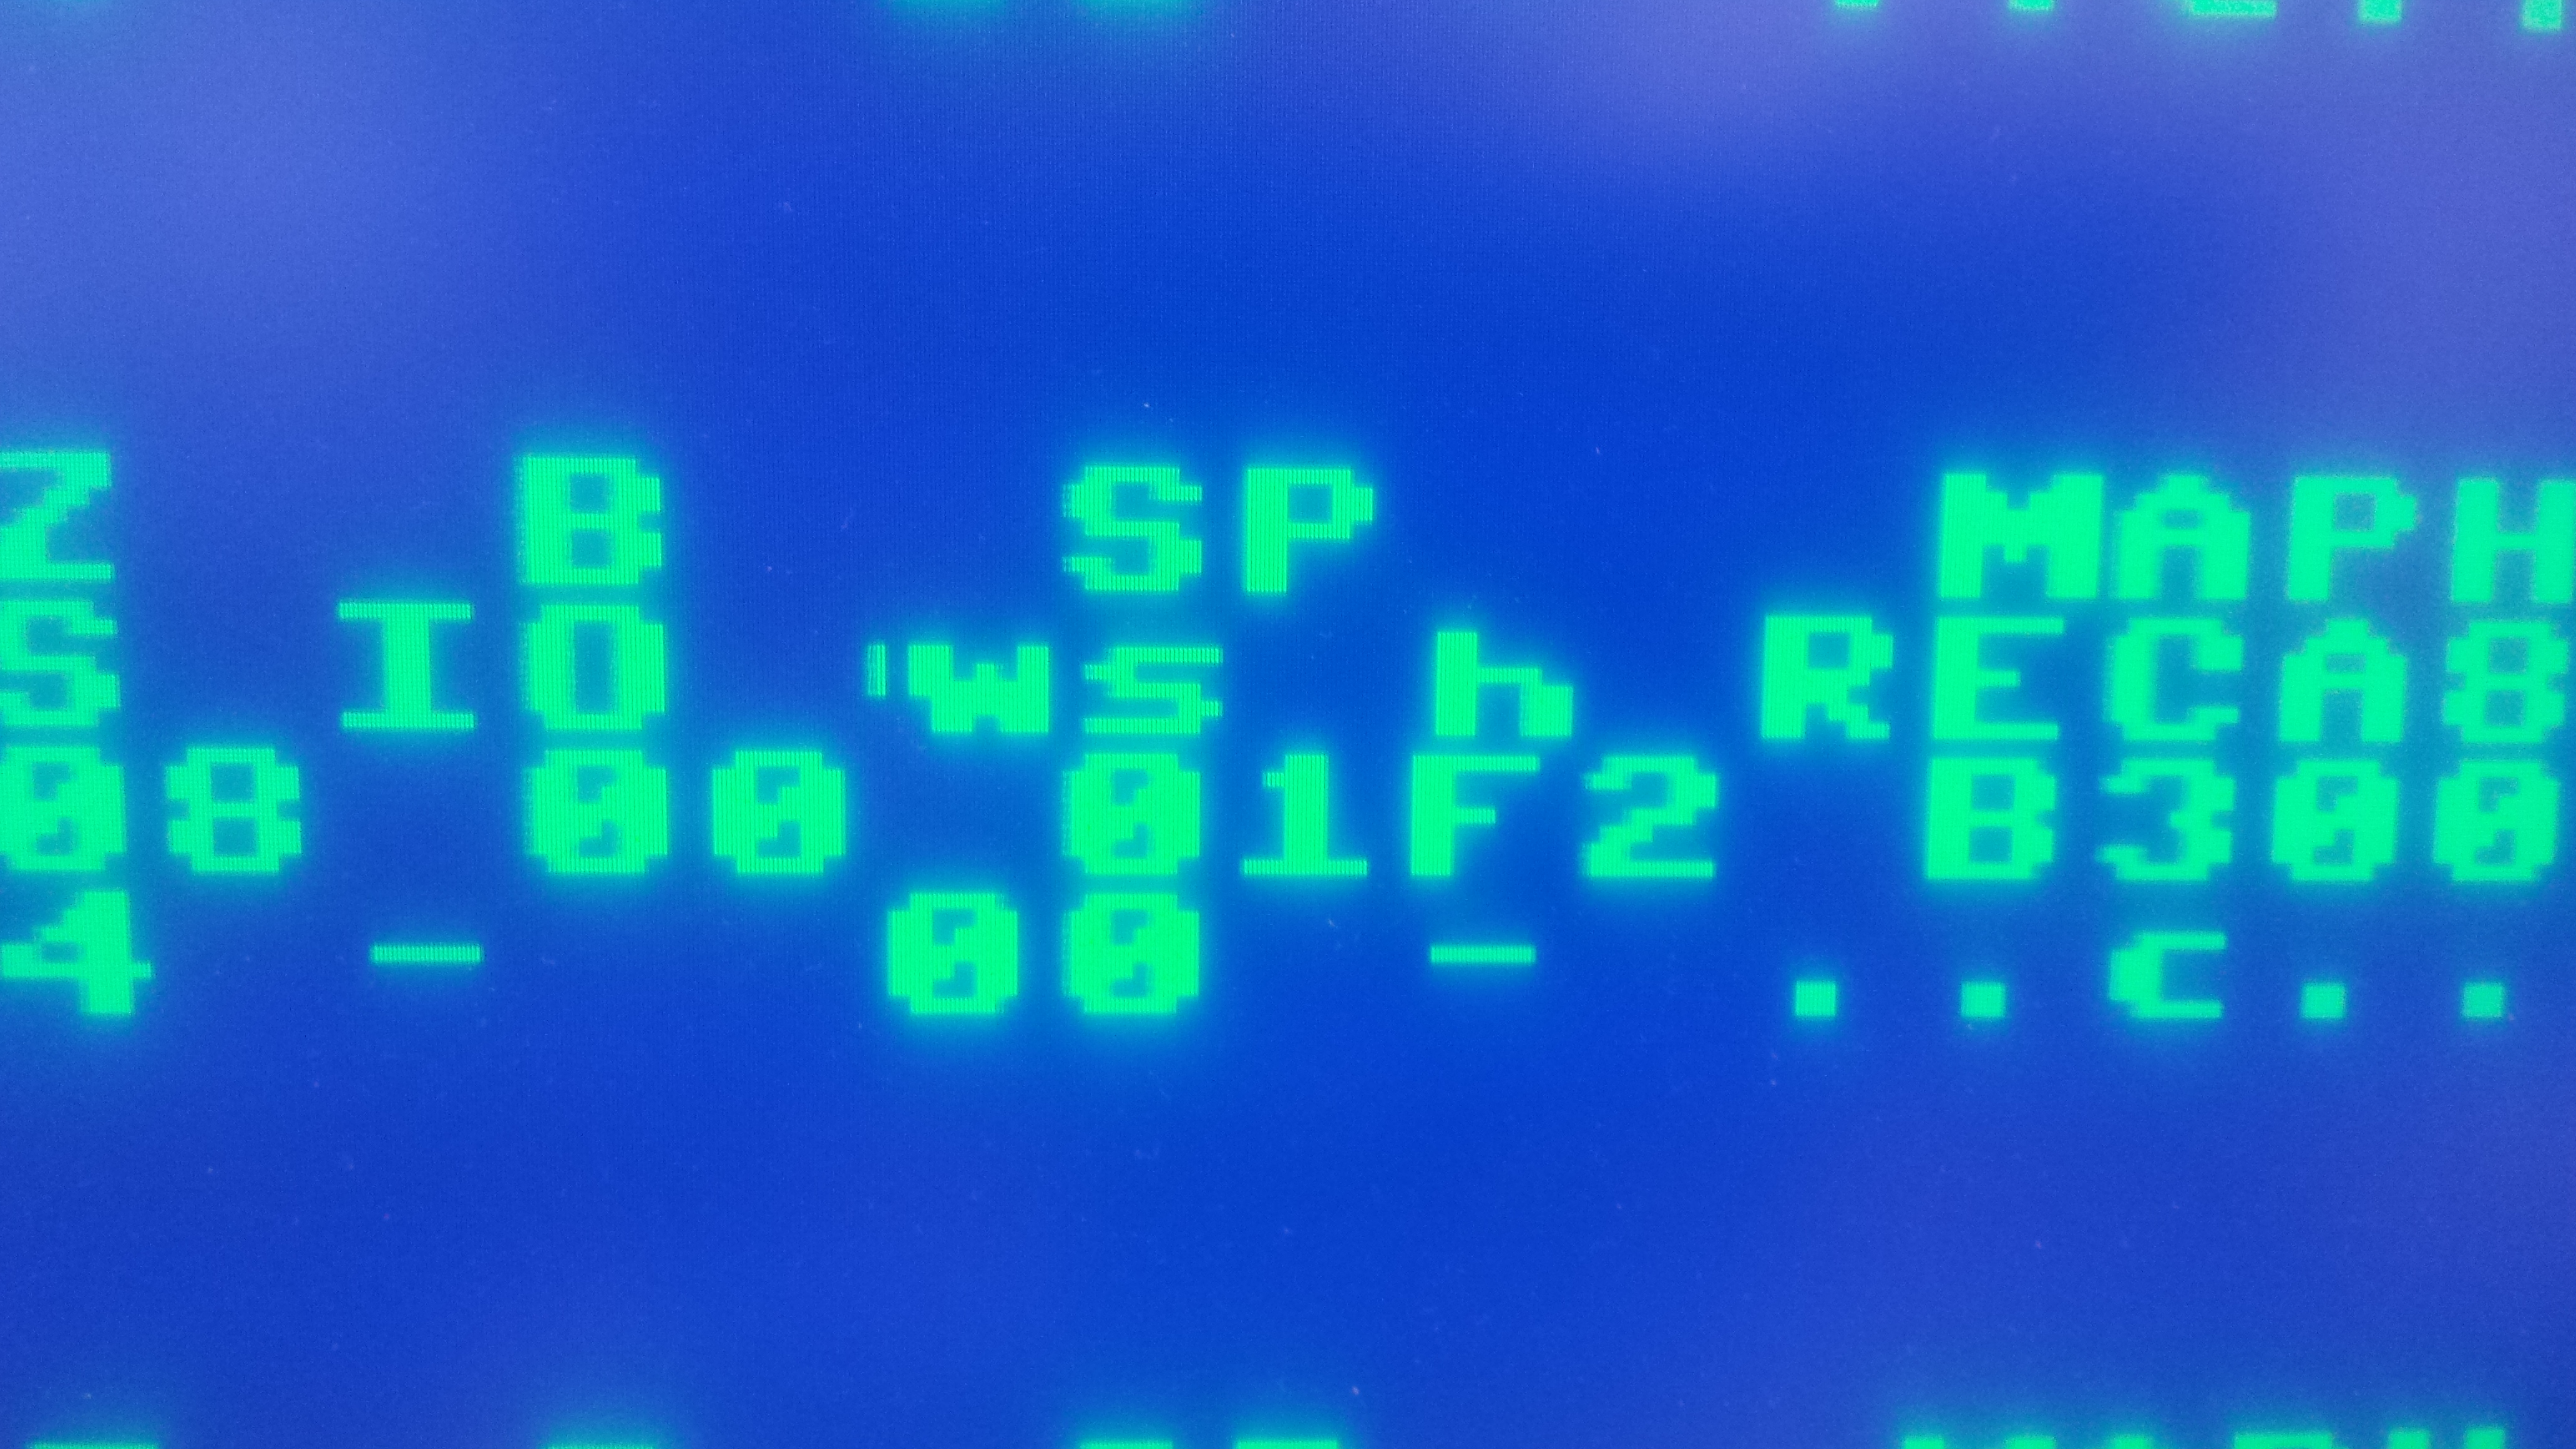
\includegraphics[width=\linewidth]{biterror}
  \caption{The matrix mode character shift.}
  \label{fig:biterror}
\end{figure}

\begin{figure}
  \centering
  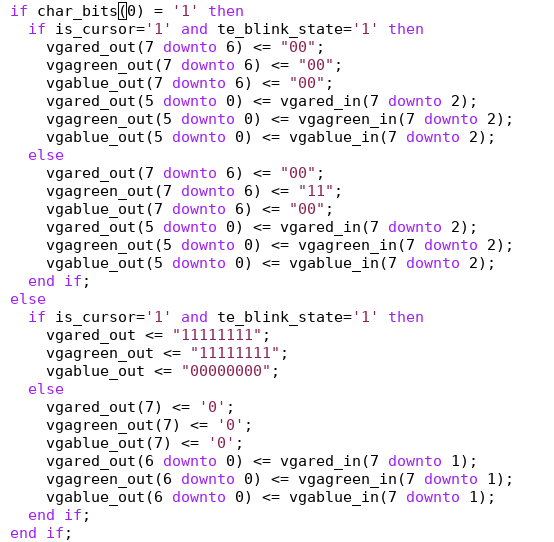
\includegraphics[width=\linewidth]{charbitstwo}
  \caption{The character bits to vga output code.}
  \label{fig:charbitstwo}
\end{figure}

\begin{figure}
  \centering
  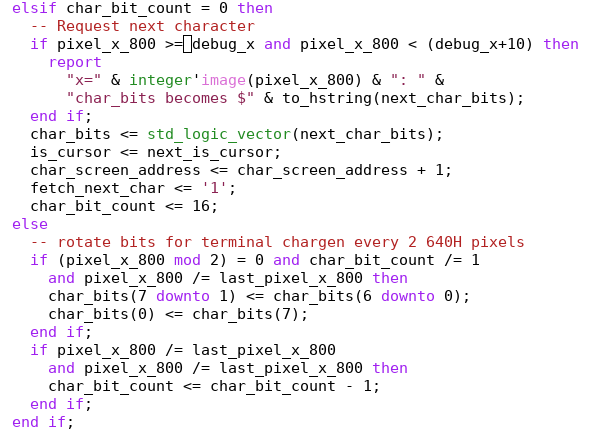
\includegraphics[width=\linewidth]{charbits}
  \caption{The character bit rotation code.}
  \label{fig:charbits}
\end{figure}

\begin{figure}
  \centering
  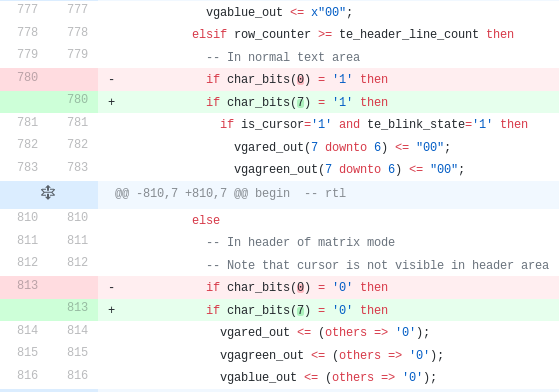
\includegraphics[width=\linewidth]{bitfix}
  \caption{The manual bit shift to counter the shifting error.}
  \label{fig:bitfix}
\end{figure}

%-----------------------------------
%	SUBSECTION 4
%-----------------------------------

\subsection{Letterbox Fixing}

\label{Ch5 Sec3 Sub4}

In collaboration with Dr. Gardner-Stephen, the junk characters seen at the bottom section of matrix mode, as seen if figure \ref{fig:letterbox}, were able to be restricted from the display. To perform this restriction of the output to the visible section of the screen, the row counter variable was used to determine if the current row was beyond the end of the matrix mode display. As seen in figure \ref{fig:letterboxfixtwo}, if the current row was beyond the end of the writeable matrix mode display, the vga input was darkened and passed out. This would hard code out any possibility of the matrix mode display being corrupted by junk characters being present in the terminal memory due to other faults.

\begin{figure}
  \centering
  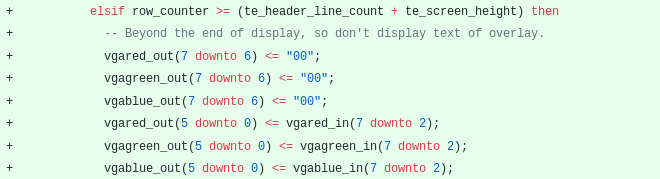
\includegraphics[width=\linewidth]{letterboxfixtwo}
  \caption{Correction to the rain compositor to stop the junk characters appearing in the lower section of the screen.}
  \label{fig:letterboxfixtwo}
\end{figure}

%-----------------------------------
%	SUBSECTION 5
%-----------------------------------

\subsection{Character Duplication}

\label{Ch5 Sec3 Sub5}

After letterbox implementation as described in section \ref{Ch5 Sec2}, a strange phenomenon occurred on the left side of the screen when in matrix mode. It appears that there is a region, about four character wide, that contains duplicates of characters from the next line. In addition to this duplicate, there appears to be smearing of the first two characters in this duplicate region. These observations can be seen in figure \ref{fig:matrixmodecharacterinputerror}. In addition to the issues with the left region, it is believed that these issues are causing the screen to become shifted to the right. As seen in figure \ref{fig:matrixmodecharacterinputerror}, the last four characters of the line are continuing past the right most visible point of the screen. 

\begin{figure}
  \centering
  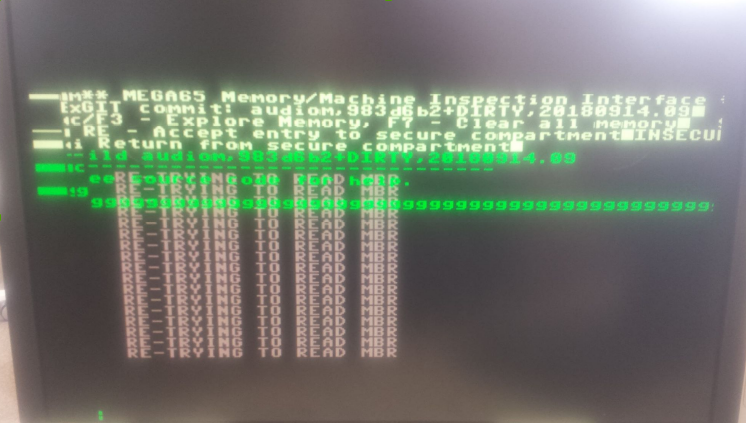
\includegraphics[width=\linewidth]{matrixmodecharacterinputerror}
  \caption{The matrix rain compositor smearing / duplication.}
  \label{fig:matrixmodecharacterinputerror}
\end{figure}
